\chapter{The Variable Library}
\label{chap:variable-library}

Variable\index{variables} in Opus and UrbanSim represent quantities of interest.  These
variables can be used in two principal ways: in specifying models and in
computing indicators\index{indicator} to assess simulation results.  For example, a
\variable{distance_to_highway} variable might be used to help predict land
values or or household location choices; and a \variable{population_density}
variable might be used in computing indicators that are useful for
evaluating simulation results.  The variable library\index{variable library} is a repository for
variables defined in the system that are accessible from the GUI\@.  Since
it provides a resource that is used throughout the GUI, we access it from
the tools menu on the menu bar at the top of the main window, as in Figure
\ref{fig:variable-library-menu}.  The screenshot in Figure
\ref{fig:variable-library-popup} shows a popup window that appears once a
user selects the variable library option on the tools menu.  Note that the
contents of it depend on what project is loaded.  In this case, we have the
eugene\_parcel project loaded, and see the variables that are initially
available in this project.

Variables are described in detail later in this manual.
Briefly for now, there are three ways to define a variable:

\begin{itemize}

\item A variable can be defined using an expression\index{expressions} written in a
  domain-specific programming language.  There is a short description of
  the language later in this chapter, and a more complete description in
  Chapter~\ref{chapter:expressions}.  In this chapter 
  we'll only be looking at defining new variables in this way.

\item A variable can also be a primary attribute of a dataset (think of
  these as columns in the input database).

\item Finally, a variable can be defined as a Python class.  This is an
  advanced option for complicated variables beyond the scope of the
  domain-specific programming language --- we'll use variables defined this
  way that are already in the library, but for now won't write any new ones.

\end{itemize}

\begin{figure}[htp]
\begin{center}
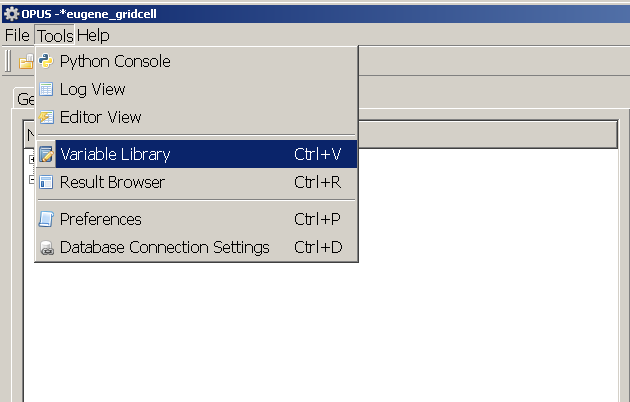
\includegraphics[scale=0.6]{part-gui/images/model-manager-variable-library-menu.png}
\end{center}
\caption{Opening the Variable Library from the ``Tools'' Menu}
\label{fig:variable-library-menu}
\end{figure}

\begin{figure}[htp]
\begin{center}
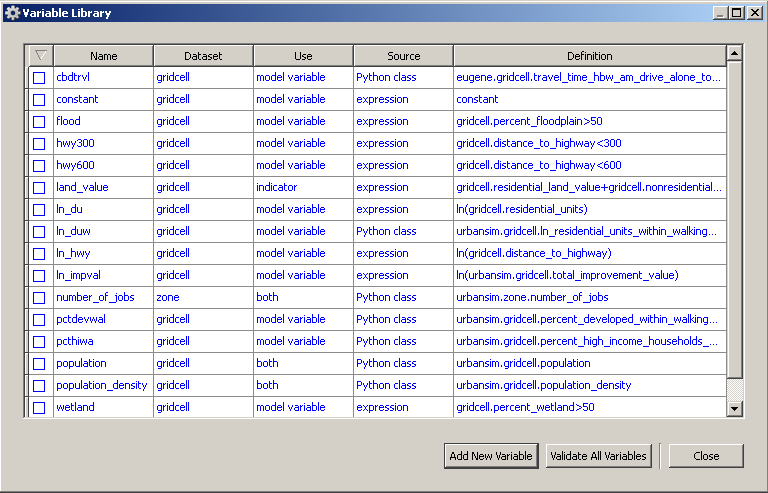
\includegraphics[scale=0.6]{part-gui/images/model-manager-variable-library-popup.png}
\end{center}
\caption{Variable Library Popup Window}
\label{fig:variable-library-popup}
\end{figure}

Note the buttons at the bottom of this window to add new variables or
validate all variables.  Adding a new variable defined as an expression is
straightforward.  There are examples of existing variables defined using
expressions in the variable library window --- look for variables with the
entry ``expression'' in the ``Source'' column.  The corresponding variable
definition is in the right-most column.  Note that this definition is
executable code --- it's not just a description.  Expressions are built up
as functions and operations applied to existing variables in the library.
For example, the expression for wetland is defined as
\variable{gridcell.percent_wetland>50}.  This defines the creation of a
true/false, or boolean, variable that is interpreted as 1 if the gridcell
has more than 50 percent coverage by wetland, 0 otherwise.  Variables are
array-valued, so we are actually computing an array of true/false values
for every gridcell with the single expression.

If you click on the add new variable button at the bottom of the variable
library window, it opens a dialog box as shown in Figure
\ref{fig:variable-library-new-variable}.  The top entry is the name you
want to use for the variable.  Let's say we want to create a new variable
that is a log of population density.  We already have a population density
variable defined by gridcell, so we can just take the log of this value.
Let's name the variable \variable{ln_population_density}, leave the middle
selection as ``expression,'' and fill in a simple expression in the
definition area: \variable{ln(gridcell.population_density)}.  We're only
going to use this variable in defining new models, not as an indicator, so
we just check the ``Will this variable be used in a model?''  box, and
leave ``Will this variable be used as an indicator?'' unchecked.  Which
boxes you check show up in the ``Use'' column of the variable library
popup window, and also determine whether the new variable appears in 
lists of variables that you can add to a model specification or use to
produce an indicator map\index{indicator map}; but don't matter for the underlying definition.

The dialog box provides two buttons at the bottom to help you check your
new variable.  The check syntax button tests whether the expression you
have entered passes the Python and expression syntax checkers -- in other
words, is it syntactically correct.  The second allows you to test whether
if you apply this expression to your available data, it can successfully
compute a result.  This is very helpful in determining whether you might
have referred to a data element that is not present, or is otherwise not
computable with your data.  In short, these two tools allow testing whether
the variables are in a state that can be computed on the available data.

\begin{figure}[htp]
\begin{center}
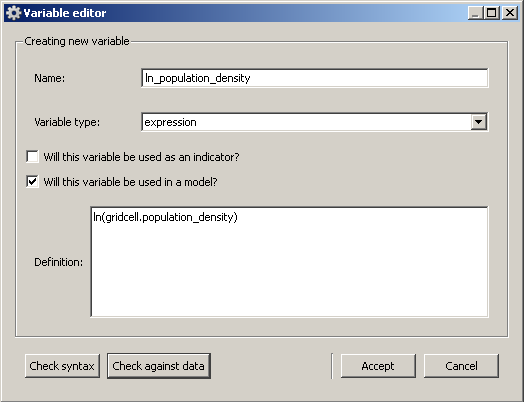
\includegraphics[scale=0.6]{part-gui/images/model-manager-variable-library-new-variable.png}
\end{center}
\caption{Adding a New Variable}
\label{fig:variable-library-new-variable}
\end{figure}

We just saw an example of using an expression to define the
\variable{ln_population_density} variable.  More generally, an expression
for a new variable will be written in terms of existing variables, where
these existing variables are referenced as a ``qualified name''\index{qualified name} consisting
of the dataset name and the variable name, for example,
\variable{gridcell.population_density}.  Or our new variable can be used in
yet another definition by writing \emph{its} qualified name:
\variable{gridcell.ln_population_density}.

In building up an expression, we can apply various functions to other
variables or subexpressions.  For subexpressions that are arrays of
floating point numbers, the available functions include \code{ln},
\code{exp}, and \code{sqrt}.  We can also use the operators \code{+},
\code{-}, \code{*}, \code{/}, and \code{**} (where \code{**} is
exponentiation).  The standard operator precedence rules apply: \code{**}
has the highest precedence, then \code{*} and \code{/}, then \code{+} and
\code{-}.

You can use constants in expressions as well, which are coerced into arrays
of the appropriate size, all filled with the constant value.  For example,
\variable{ln(2*gridcell.population_density)} is an array, consisting of the
logs of 2 times the population density of each grid cell. 

Two subexpressions\index{subexpressions} that are arrays of integers or floats can be compared
using one of the relational operators \code{<}, \code{<=}, \code{==},
\code{>=}, \code{>}, or \code{!=} (not equal).  We saw an an example of
using a relational operation in the \variable{gridcell.percent_wetland>50}
expression.  \variable{gridcell.percent_wetland} denotes an array of
integers, one for each gridcell.  The constant 50 gets coerced to an array
of the same length, and then the \code{>} operator compares the
corresponding elements, and returns an array of booleans.
